% many codes were copied from https://github.com/cuhk-ri/cuhk-thesis
% Revised by CHEN, Yuelong (yuelong.chen.btr@gmail.com)


\documentclass[12pt,a4paper,twoside]{report}
\usepackage{amsmath,amsthm,amssymb,fancyhdr,url}
\usepackage{fontspec}
\usepackage[scheme=plain]{ctex}

%=======================================================
\usepackage{latexsym}
\usepackage{xcolor}
\usepackage{amsmath}
\usepackage{amssymb}
\usepackage{amsfonts}
\usepackage{url}
\usepackage{amsthm}
\usepackage{tocbibind}
\usepackage{bm}
\usepackage{mathtools}
\usepackage{graphicx}

\def\degree#1{\def\degree{#1}}
\def\programme#1{\def\programme{#1}}
\def\supervisor#1{\def\supervisor{#1}}
\def\thesistitle#1{\def\thesistitle{#1}}
\def\thesistitlezh#1{\def\thesistitlezh{#1}}
\def\authorname#1{\def\authorname{#1}}
\def\submitdate#1{\def\submitdate{#1}}
\def\institution#1{\def\institution{#1}}
\def\committee#1{\def\committee{#1}}
\def\thecommittee#1{\def\thecommittee{#1}}

\def\coverpage{
  % no page number for the cover page
  \thispagestyle{empty}

  \vspace*{2cm}
  \begin{center}
    \LARGE {\bf \thesistitle}

    \vskip 1cm
    \large \authorname

    \vskip 1cm
    \large
  % both Fulfilment and Fulfillment are correct
    A Thesis Submitted in Partial Fulfilment \\
    of the Requirements for the Degree of \\
    \degree \\
    in \\
    \programme \\

    \vfill
    \large \institution \\
    \submitdate
  \end{center}

  \newpage

  \thispagestyle{empty}
  \vspace*{10mm}
  \begin{center}
    \vfill
    \large
    \underline{\bf Thesis Assessment Committee}
    \vskip 1.5cm
    \committee
    \vfill
  \end{center}
  \normalsize
  \newpage
}

%=======================================================

\def\abstractpage{
  \chapter*{Abstract}
  \addcontentsline{toc}{chapter}{Abstract}

  of thesis entitled: \\
  \indent \underline{\thesistitle} \\
  Submitted by \authorname \\
  for the degree of \degree \\
  at \institution~in \submitdate

  \vskip 1cm \noindent
  Put your abstract text here.

  \vfill

  \vspace*{1.5cm}
  \chapter*{摘要}
  \addcontentsline{toc}{chapter}{摘要}
  \noindent \underline{\thesistitlezh}
  \vskip 1cm
  此为摘要。

  \clearpage
}

%=======================================================

\def\acknowledgementpage{%
  \chapter*{Acknowledgement}
  \addcontentsline{toc}{chapter}{Acknowledgement}
  I would like to thank my supervisor Prof. 

  \newpage
}

%=======================================================

\def\dedicationpage{%
  \vspace*{1cm}
  \vfill
  \begin{center}
    Dedicated to those who risked their life fighting against \mbox{COVID-19}.

  \end{center}
  \vfill
  \newpage
}

%=======================================================

\newcommand{\snote}[2]{%
  \vspace*{3mm}
  \begin{center}
    \framebox[13.6cm][t]{%
      \hspace*{2mm}
      \parbox[t]{12.8cm}{%
        \vspace*{2mm}
        \centerline{\bf #1}\vspace*{-2mm}
        \rule{12.8cm}{0.4mm}
        \\#2
        \vspace*{3mm}
      }
    }
  \end{center}
  \vspace*{3mm}
}

\newcommand{\chapterend}{
  \vfill
  \noindent\rule{\textwidth}{0.5mm} \\
  \noindent{\large\bf $\Box$ End of chapter.}
}

\newcommand{\reading}[1]{
  \vfill
  \noindent {\bf $\equiv$ Readings:}  #1
}


\theoremstyle{remark} \newtheorem{remark}{Remark}
\theoremstyle{remark} \newtheorem*{note}{Note}
\theoremstyle{definition} \newtheorem{assumption}{Assumption}
\theoremstyle{definition} \newtheorem*{problem}{Problem}
\theoremstyle{definition} \newtheorem{definition}{Definition}
\def\bbR{\mathbb{R}}
\def\bbN{\mathbb{N}}
\def\bR{\mathbf{R}}
\def\bx{\mathbf{x}}
\def\bz{\mathbf{z}}
\def\bfe{\mathbf{e}}
\def\br{\mathbf{r}}
\def\bT{\mathbf{T}}
\def\bp{\mathbf{p}}
\def\bq{\mathbf{q}}
\def\ba{\mathbf{a}}
\def\bg{\mathbf{g}}
\def\bv{\mathbf{v}}
\def\bu{\mathbf{u}}
\def\bl{\mathbf{l}}
\def\bJ{\mathbf{J}}
\def\bH{\mathbf{H}}
\def\bI{\mathbf{I}}
\def\bQ{\mathbf{Q}}
\def\bK{\mathbf{K}}
\def\bM{\mathbf{M}}
\def\bzero{\mathbf{0}}
\def\caN{\mathcal{N}}
\def\caX{\mathcal{X}}
\def\caG{\mathcal{G}}
\def\bOmega{\bm\Omega}
\def\bomega{\bm\omega}
\def\bSigma{\bm\Sigma}
\def\bsigma{\bm\sigma}
\def\bvarsigma{\bm\varsigma}
\def\btheta{\bm\theta}
\def\bdelta{\bm\delta}
\def\bDelta{\bm\Delta}
\def\bPhi{\bm\Phi}
\def\bmV{\bm V}
\def\bxi{\bm\xi}
\def\brho{\bm\rho}
\def\bnu{\bm\nu}
\def\bmeta{\bm\eta}
\def\bvarrho{\bm\varrho}
\def\bvarrho{\bm\varrho}
\def\det{\mathrm{det}}
\def\tr{\mathrm{tr}}
\def\trans{^\mathrm{T}}
\def\diag{\mathrm{diag}}
\def\adj{\mathrm{adj}}
\def\inv{^{-1}}
\def\caJ{\mathcal{J}}
\def\caT{\mathcal{T}}
\def\bfb{\mathbf{b}}
\def\bmb{\bm b}
\def\Exp{\mathrm{Exp}}
\def\Log{\mathrm{Log}}
\def\half{\frac{1}{2}}
\def\SO{\mathrm{SO}}
\def\SE{\mathrm{SE}}
\def\sefr{\mathfrak{se}}
\def\sofr{\mathfrak{so}}
\def\tk{ {} }

\def\argmin{\operatorname*{arg\,min}}
\def\argmax{\operatorname*{arg\,max}}

\newcommand{\Norm}[1]{
    \left\| #1 \right\|
}
\newcommand{\norm}[1]{
    \left| #1 \right|
}
\newcommand{\deriv}[2]{
	\frac{\mathrm{d}\, #1}{\mathrm{d}\, #2}
}
\newcommand{\pderiv}[2]{
  \frac{\partial\, #1}{\partial\, #2}
}
\newcommand{\halfof}[1]{
  \frac{#1}{2}
}
\newcommand{\vIm}[1]{
\left[#1\right]_\Im
}
%=======================================================

% margins and spacing required by CUHK Grad-School
% 4 cm margin for binding edge, 2.5 cm for outer edge:
\usepackage[inner=4cm,outer=2.5cm]{geometry}
\usepackage{setspace}

% 1.5 line spacing for normal texts:
\setstretch{1.5}
% avoid too much space automatically padded between paragraphs to fill a page:
\raggedbottom

% personally imported packages and customization
\usepackage[mono=false]{libertine} % I personally favour this font
\usepackage{subfig}
\usepackage{tikz}
\usepackage{pgfplots}
\graphicspath{{figures/}}
\usepackage[authoryear,square,comma,numbers]{natbib} % citation style management
%\def\cite{\citep}
% CUHK has no limitations on bibliography style, use your favor.
%\bibliographystyle{ieeetr} % for 'nubmers' citation style
\bibliographystyle{apalike} % for 'authoryear' citation style
\usepackage[colorlinks=true,linkcolor=blue,citecolor=magenta]{hyperref}



%=======================================================
\begin{document}

\thesistitle{My templates}
\thesistitlezh{香港中文大学学位论文标题} % CUHK 对简繁体不作要求
\authorname{CHEN, Yuelong}
\degree{Doctor of Philosophy}
\programme{Mechanical and Automation Engineering}
\institution{The Chinese University of Hong Kong}
\submitdate{March 1874}
\committee{
	Professor ZHANG San (Chair)\\
	Professor LI Si (Thesis Supervisor)\\
	Professor WANG Wu (Thesis Co-supervisor)\\
	Professor ZHAO Liu (Committee Member)\\
	Professor WHO Ever (External Examiner)
}
\coverpage

%=======================================================
\pagenumbering{roman}
\abstractpage
%=======================================================
\acknowledgementpage
%=======================================================
\tableofcontents
\listoffigures
\listoftables


\chapter*{Symbols and Acronyms}
\addcontentsline{toc}{chapter}{Symbols and Acronyms}

In general, we denote a scalar by an italic lower case letter,
a vector by a roman lower case bold letter,
and a matrix by a roman upper case bold letter respectively, e.g.,
$a \in \bbR$, $\mathbf{v} \in \bbR^n$ and $\mathbf{M} \in \bbR^{p \times q}$, with any exceptions to be mentioned in the context case by case.

Specifically, the components of any vector ${\bf v} \in \bbR^2$ or ${\bf v}\in \bbR^3$ are written as $[v_x\,v_y]^T$ or $[v_x\,v_y\,v_z]^T$.

An identity matrix is written as $\bI$. Specifically, an $n\times n$ identity matrix is written as $\bI_n$.
A zero matrix or vector is written as ${\bf 0}$. Specifically, an $m\times n$ zero matrix is written as ${\bf 0}_{m\times n}$.

$\check{(\cdot)}$ denotes the prior of any quantity, while $\hat{(\cdot)}$ denotes the posterior.

Specialized symbols and major acronyms are defined as follows:

\newpage

\noindent
$\bR \in$ SO(3) \hfill a $3\times 3$ rotation matrix \\
$\bT \in$ SE(3) \hfill a $4 \times 4$ homogeneous transformation matrix\\
$\bp \in \bbR^3$ \hfill a 3D translational vector \\
$\bq=[q_x \, q_y \, q_z \, q_w ]^T$ \hfill a Hamilton quaternion, with $q_w$ being the real part \\
$[\bq]_\Im=[q_x\,q_y\,q_z]^T$ \hfill the imaginary vector part of $\bq$\\
$\otimes$ \hfill multiplication of quatertions \\
$\bm\theta \in \bbR^3$ \hfill a rotation vector \\
$\bl \in \bbR^3$ \hfill the 3D position of a landmark point \\
$\bv \in \bbR^3$ \hfill  translational velocity \\
$\ba \in \bbR^3$ \hfill  translational acceleration \\
$\bm\omega \in \bbR^3$ \hfill  angular velocity \\
${\bf u} \in \bbR^2$ \hfill 2D position in image coordinates \\
$p(\cdot)$ \hfill the probability density function (PDF) \\
$E(\cdot)$ \hfill  the expectation \\
$\bm\Sigma$ \hfill a covariance matrix \\
$\bm\Omega$ \hfill an information matrix \\
$\caN(\bar\bx,\bSigma)$ \hfill a normal distribution with mean $\bar\bx$ and covariance $\bSigma$ \\
${\bm\eta}$ \hfill a noise vector \\
${\bf e}(\cdot)$ \hfill an error/residual function \\
$\bJ$ \hfill a Jacobian matrix \\
$\bH$ \hfill a Hessian matrix \\
$\bJ_\ell$ \hfill left Jacobian of SO(3) \\
$\caJ_\ell$ \hfill left Jacobian of SE(3) \\
$\caT$ \hfill adjoint of SE(3)\\
$\tr(\cdot)$ \hfill trace of a matrix \\
$\det(\cdot)$ \hfill determinant of a matrix \\



\newpage
\noindent
BA        \hfill bundle adjustment                       \\
BoW       \hfill Bags of Words                           \\
DoF       \hfill degree of freedom                       \\
EKF       \hfill extended Kalman filter                  \\
GPS       \hfill Global Positioning System               \\
GN        \hfill Gauss-Newton                            \\
IMU       \hfill inertial measurement unit               \\
KF        \hfill Kalman filter                           \\
LM        \hfill Levenberg-Marquardt                     \\
MAP       \hfill maximum a posteriori                    \\
PF        \hfill partical filtering                      \\
RANSAC    \hfill random sample consensus                 \\
SfM       \hfill structure from motion                   \\
SLAM      \hfill simultaneously localization and mapping \\
MSCKF     \hfill multi-state constraint Kalman filter    \\
ToF       \hfill Time-of-Flight                          \\
UKF       \hfill unscended Kalman filter                 \\
V-SLAM    \hfill visual SLAM                             \\
VINS      \hfill visual inertial navigation system       \\
VIF       \hfill visual inertial fusion                  \\
VIO       \hfill visual inertial odometry                \\
VO        \hfill visual odometry                         \\


%=======================================================

\newpage
\setcounter{page}{0}
\pagenumbering{arabic}
\pagestyle{headings}
%=======================================================
%insert the chapters
\chapter{Introduction}
\label{chap:intro}
\def\summarynote{
  This chapter introduces the background and some related work of \ldots\ldots.
  
  It also lists the contributions and sketches the outline of the thesis.
}
\snote{Summary}{\summarynote}

\section{Background}
\label{sec:intro-background}


\section{Related Work}
\label{sec:intro-related}


\section{Contributions}
\label{sec:intro-contri}


\section{Organization}
\label{sec:intro-orga}

The remainder of the thesis is organized as follows.

\snote{Summary}{\summarynote}
\chapterend


\chapter{Topic One}
\label{chap:topic-one}
\def\summarynote{
  This chapter presents \ldots\ldots
}
\snote{Summary}{\summarynote}

\section{Figure Example with tikz}
\label{sec:figure-tikz}

Check Figure \ref{fig:tikz}.

\begin{figure}[h]
  \centering
  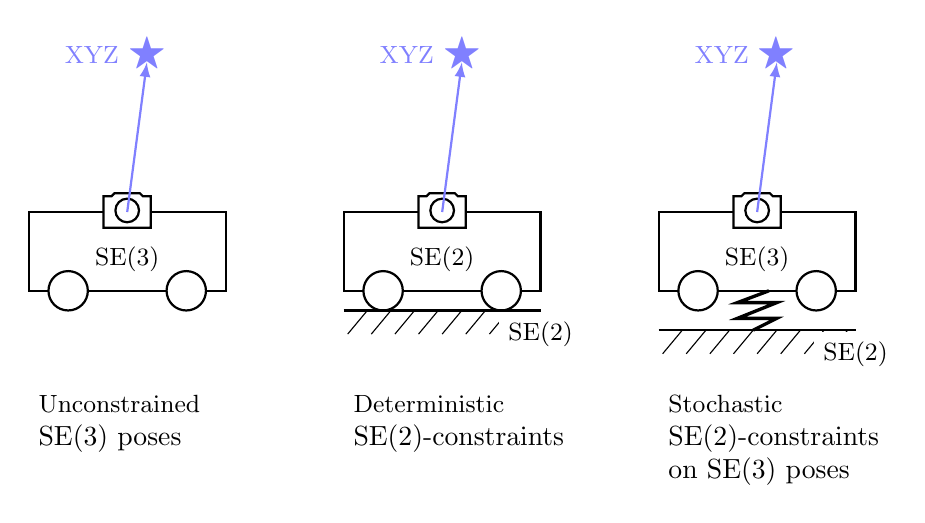
\begin{tikzpicture}[>=latex,scale=1.0,
  ]

  \def\cameraicon#1#2{
    \begin{scope}[shift={#1}, rotate=#2]
      \draw[thick,fill=white] (-0.3,-0.2) -- (0.3,-0.2) -- (0.3,0.2) -- (0.2,0.2) --
      (0.16,0.24) -- (-0.16,0.24)--(-0.2,0.2)--(-0.3,0.2)--cycle;
      \draw[thick,fill=white] (0,0.02) circle [radius=0.15];
    \end{scope}
  }
  % \draw[gray!50,step=0.5] (0,0) grid (12,6);
  \foreach \x in {0.5,4.5,8.5}
  {
    \draw[thick] (\x,2) rectangle (\x+2.5,3);
    \draw[thick,fill=white] (\x+0.5,2) circle [radius=0.25];
    \draw[thick,fill=white] (\x+2,2) circle [radius=0.25];
    \draw[blue!50] (\x+1.5,5) node {\Large $\bigstar$};
    \draw[blue!50] (\x+0.8,5) node {\small XYZ};
    \cameraicon{(\x+1.25,3)}{0}
    \draw[blue!50,thick,->] (\x+1.25,3) -- (\x+1.5,4.9);
  }
  \foreach \x in {1,2,3,4,5,6,7,8}
  {
    \draw (4.5+\x*0.30,1.75) -- +(-0.25,-0.3);
    \draw[xshift=4cm,yshift=-0.25cm] (4.5+\x*0.30,1.75) -- +(-0.25,-0.3);
  }
  \draw[] (1.75,2.4) node {\small SE(3)};
  \draw[] (5.75,2.4) node {\small SE(2)};
  \draw[] (9.75,2.4) node {\small SE(3)};
  \draw[yshift=0.25cm] (7,1.2) node[fill=white] {\small SE(2)};
  \draw[xshift=4cm] (7,1.2) node[fill=white] {\small SE(2)};
  \draw[thick] (4.5,1.75) -- (7,1.75);
  \draw[thick,xshift=4cm,yshift=-0.25cm] (4.5,1.75) -- (7,1.75);
  \draw[very thick] (9.7,1.5) -- (10,1.65) -- (9.5,1.65) -- (10,1.85) -- (9.5,1.85) --(9.9,2);

  \draw (0.5,0.8) node[below right,align=left] {\small Unconstrained\\ SE(3) poses};
  \draw[xshift=4cm] (0.5,0.8) node[below right,align=left] {\small Deterministic\\ SE(2)-constraints};
  \draw[xshift=8cm] (0.5,0.8) node[below right,align=left] {\small Stochastic\\ SE(2)-constraints\\ on SE(3) poses};

\end{tikzpicture}

  \caption{Plotting figures using tikz like this.}
  \label{fig:tikz}
\end{figure}


\section{Figure Example with pgfplots}
\label{sec:figure-pgfplots}

Check Figure \ref{fig:pgfplots}.

\begin{figure}[h]
  \centering
  % \documentclass{standalone}
% \usepackage{tikz}
% \usepackage{pgfplots}

% \begin{document}

\begin{tikzpicture}
\begin{axis}[
    axis equal=true,
    small,
    width=10cm,
    height=6cm,
    title={Trajectories: \textit{Dataset Room}},
    xlabel={x [m]},
    ylabel={y [m]},
    grid=major,
    grid style={dotted},
    % xmin=0,xmax=85,
    % grid=major,
    legend style={
      at={(0.6,0.75)},
      font=\footnotesize,
    },
]
\addplot [black,thick] table {figures/ba-r4-007.traj-odoerrTruetrj.dat};
\addplot [red,densely dashed] table {figures/ba-r4-007.traj-odoerrOdometrytrj.dat};
\addplot [blue,thin] table {figures/ba-r4-007.traj-odoerrORB-SLAMtrj.dat};
\addplot [green!50!black!80,thick] table {figures/ba-r4-007.traj-odoerrOurstrj.dat};
\legend{Truth,Odometry,ORB-SLAM, Ours},
\end{axis}
\end{tikzpicture}
% \end{document}

  \caption{Plotting figures using pgfplots like this.}
  \label{fig:pgfplots}
\end{figure}

\clearpage
\snote{Summary}{\summarynote}
\chapterend

\chapter{Topic Two}
\label{chap:topic-two}
\def\summarynote{
  This chapter presents \ldots\ldots
}
\snote{Summary}{\summarynote}

\section{Citation Example}
\label{sec:cite}

Bibliography data is put in database.bib.
Cite like this \cite{craigbook} \cite{barfoot2017state}.

\snote{Summary}{\summarynote}
\chapterend

\chapter{Conclusion}
\label{chap:con}

\snote{Summary}
{
This chapter summarizes the contributions of this thesis, and proposes some potential directions for future work.
}

\section{Contributions}

\section{Future Work}

\chapterend



%=======================================================
\appendix
\chapter{Proof of Propositions} 

\chapterend

\chapter{Publication List}


\chapterend


%=======================================================
\newpage
% CUHK recommend single-spaced references
\setstretch{1}
\bibliography{reference}

\end{document}

